\documentclass{article}
\usepackage{tikz}
\usetikzlibrary{shapes.geometric}

\begin{document}

\begin{figure}[h]
    \centering
    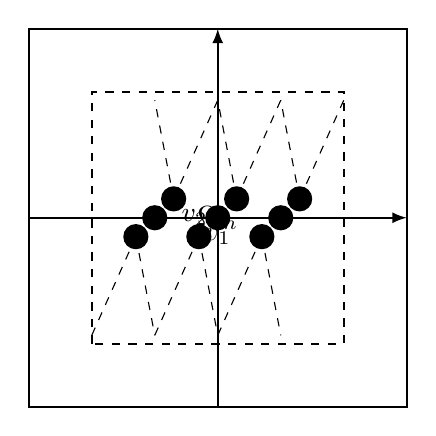
\begin{tikzpicture}[scale=0.8]

        % Define the main cube (Omega)
        \draw[thick] (-3,-3) rectangle (3,3);

        % Define the subdomain Omega_m
        \draw[thick,dashed] (-2,-2) rectangle (2,2);
        \node at (0,0) {$\Omega_m$};

        % Draw the vectors v_1 and v_2 for reference
        \draw[-latex,thick] (0,-3) -- node[below]{$v_1$} (0,3);
        \draw[-latex,thick] (-3,0) -- node[left]{$v_2$} (3,0);

        % Draw the hexagonal pattern within Omega_m
        \foreach \x in {-1,0,1} {
            \foreach \y in {-1,0,1} {
                \pgfmathsetmacro{\angle}{60*\y}
                \pgfmathtruncatemacro{\colorIndex}{mod(\x+\y, 2)}
                \ifnum\colorIndex=0
                    \definecolor{myColor}{RGB}{0,255,0} % Green
                \else
                    \definecolor{myColor}{RGB}{255,0,0} % Red
                \fi
                \fill[\myColor] (\x+.3*\y, .3*\y) circle (0.2cm);
                \draw[dashed] (\x+.3*\y, .3*\y) -- ({\x+.5*\y + cos(\angle)}, {\y + sin(\angle)});
                \draw[dashed] (\x+.3*\y, .3*\y) -- ({\x+.5*\y - cos(\angle)}, {\y + sin(\angle)});
            }
        }

    \end{tikzpicture}
    \caption{Elongated Honeycomb. Here, the domain $\Omega$ is a cube and the decomposing subdomains $\Omega_m$'s are also cubes. In this figure, we display the sections (of square form) of $\Omega$ and $\Omega_m$'s. Each $\Omega_m$ contains 2 particles, located at the points $z_{m_{1}}$ and $z_{m_{2}}$, $m=1, .2... M$, (one is green and the other one red colored). The vector formed by each two points is characterized by the angle of the Honeycomb element.}
    \label{fig:ElongatedHoneycomb}
\end{figure}

\end{document}